

In this section, we study the generalization ability of the two-layer neural network $f_{\mat W(k), \vect a}$ trained by GD.


First, in order for optimization to succeed, i.e., zero training loss is achieved,
we need a \emph{non-degeneracy} assumption on the data distribution, defined below:
\begin{defn} \label{def:non-degenerate distribution}
	A distribution $\calD$ over $\R^d \times \R$ is $(\lambda_0, \delta, n)$-non-degenerate, if for $n$ i.i.d. samples $\{(\vect x_i, y_i)\}_{i=1}^n$ from $\calD$, with probability at least $1-\delta$ we have $\lambda_{\min}(\mat H^\infty) \ge \lambda_0 >0$.
\end{defn}
\begin{rem}
	Note that as long as no two $\vect x_i$ and $\vect x_j$ are parallel to each other, we have $\lambda_{\min}(\mat H^\infty) > 0$. (See~\citep{du2018provably}).
	For most real-world distributions, any two training inputs are not parallel.
\end{rem}

Our main theorem is the following:
\begin{thm}\label{thm:main_generalization}
	Fix % an error parameter $\epsilon>0$ and 
	a failure probability $\delta \in (0, 1)$.
	Suppose our data $S = \left\{(\vect x_i,  y_i)\right\}_{i=1}^n$ are i.i.d. samples from a $(\lambda_0, \delta/3, n)$-non-degenerate distribution $\calD$, and $\kappa = O\left( \frac{ \lambda_0 \delta}{ n} \right), m\ge \kappa^{-2} \poly\left(n, \lambda_0^{-1}, \delta^{-1} \right)  $.
	Consider any loss function $\ell: \R\times\R \to [0, 1]$ that is $1$-Lipschitz in the first argument such that $\ell(y, y)=0$.
	Then with probability at least $1-\delta$ over the random initialization and the training samples, the two-layer neural network $f_{\mat W(k), \vect a}$ trained by GD for $k\ge \Omega\left( \frac{1}{\eta\lambda_0} \log\frac{n}{\delta} \right)$ iterations has population loss $L_\calD(f_{\mat W(k), \vect a}) = \E_{(\vect x, y)\sim\calD}\left[ \ell(f_{\mat W(k), \vect a}(\vect x), y) \right]$ bounded as:
	\begin{equation} \label{eqn:main_generalization}
	L_\calD(f_{\mat W(k), \vect a}) \le \sqrt{\frac{2\vect{y}^\top \left(\mat{H}^{\infty}\right)^{-1}\vect{y}}{n}}  + O\left( \sqrt{\frac{\log\frac{n}{\lambda_0\delta}}{n}} \right) .
	%\sqrt{\frac{2 \vect y^\top (\mat H^\infty)^{-1}\vect y }{n}} + 3 \sqrt{\frac{\log(6/\delta)}{2n}} + \epsilon.
	\end{equation}
	%Suppose $\mu$ satisfies that there exists a function $\lambda_{\mu}: \mathbb{R}\rightarrow \mathbb{R}$ such that with probability at least $1-\delta_1$, $\lambda_{\min}(\mat{H}^\infty) \ge \lambda_{\mu}(\delta_1)$.\simon{better way of stating this assumption?}
%	We let $L_{tr}(k) = \frac{1}{n}\sum_{i=1}^{n}\ell(f(\mat{W}(k),\vect{a},\vect{x}_i),y_i)$ and $L_{te}(k) = \expect_{(\vect{x},y) \sim \mu }\left[\ell(f(\mat{W}(k),\vect{a},\vect{x}),y)\right]$.
%	Then if we set $m = \poly(n,\epsilon,1/\lambda_{\mu}(\delta_1),1/\delta_2)$ we have with failure probability at most $(\delta+\delta_1)$ over the training samples and with failure probability at most  $\delta_2$ over the random initialization, for $k=0,1,\ldots$\begin{align}
%	&L_{te}(k)-L_{tr}(k) \nonumber\\
%	\le &2\rho\sqrt{\frac{ \left(\vect{y}^\top \left(\mat{H}^\infty\right)^{-1}\vect{y}\right) \tr\left(\mat{H}^{\infty}\right)+\log (\delta^{-1})}{n}}+ \epsilon . \label{eqn:main_generalization}
%	\end{align}
\end{thm}


The proof of Theorem~\ref{thm:main_generalization} is given in Appendix~\ref{app:proof_generalization} and we sketch the proof in Section~\ref{sec:proof_sketch_generalization}.

Note that in Theorem~\ref{thm:main_generalization} there are three sources of possible failures: (i) failure of satisfying $\lambda_{\min}(\mat H^\infty) \ge \lambda_0$, (ii) failure of random initialization, and (iii) failure in the data sampling procedure (c.f. Theorem~\ref{thm:rad_generalization}). We ensure that all these failure probabilities are at most $\delta/3$ so that the final failure probability is at most $\delta$.

%$\delta$ represents the failure probability of the sampling procedure (c.f. Theorem~\ref{thm:rad_generalization}).
%$\lambda_{\mu}(\cdot)$ is a function that depends on the distribution $\mu$ and characterizes the Gram matrix least eigenvalue given a tolerance failure probability $\delta_1$.
%In Appendix we give justification on the existence of $\lambda_{\mu}(\cdot)$.
%Lastly, we use $\delta_2$ to characterize the failure probability from random initialization.
%Similar to $\epsilon$, both $\delta_1$ and $\delta_2$ can be arbitrarily small if we set $m$ large enough.

As a corollary of Theorem~\ref{thm:main_generalization}, for binary classification problems (i.e., labels are $\pm1$), we can show that \eqref{eqn:main_generalization} also bounds the \emph{population classification error} of the learned classifier. 
See Appendix~\ref{app:proof_generalization} for the proof.
\begin{cor} \label{cor:binary-classification-generalization}
	Under the same assumptions as in Theorem~\ref{thm:main_generalization} and additionally assuming that $y\in\{\pm1\}$ for $(\vect x, y)\sim\cD$, with probability at least $1-\delta$, the population classification error $L_\calD^{01}(f_{\mat W(k), \vect a}) = \Pr_{(\vect x, y)\sim\calD}\left[ \sgn\left(f_{\mat W(k), \vect a}(\vect x) \right) \not= y \right]$ is bounded as:
	\begin{equation*} 
	L_\calD^{01}(f_{\mat W(k), \vect a})  \le \sqrt{\frac{2\vect{y}^\top \left(\mat{H}^{\infty}\right)^{-1}\vect{y}}{n}}  + O\left( \sqrt{\frac{\log\frac{n}{\lambda_0\delta}}{n}} \right) .
	\end{equation*}
\end{cor}

Now we discuss our generalization bound.
The dominating term in \eqref{eqn:main_generalization} is:
\begin{equation}
\sqrt{\frac{ 2 \vect{y}^\top \left(\mat{H}^\infty\right)^{-1}\vect{y} }{n}}. \label{eqn:complexity}
\end{equation}
This can be viewed as a \emph{complexity measure of data} that one can use to predict the test accuracy of the learned neural network.
Our result has the following advantages:
(i) our complexity measure~\eqref{eqn:complexity} can be directly computed given data $\{(\vect x_i, y_i)\}_{i=1}^n$, without the need of training a neural network or assuming a ground-truth model;
(ii) our bound is completely independent of the network width $m$.
% (iii) our theorem does not require early stopping of optimization as in~\cite{allen2018learning}.

%Importantly, this complexity measure only depends on the labels $\vect{y}$ and the Gram matrix $\mat{H}^\infty$ which is induced by the input data and the network architecture.
%Comparing with existing generalization bound, our theorem is in dependent of number of parameters in contrast to classical VC-dimension theory based theory and our theorem does not depends on the norm of learned matrices as in recent work.
%Furthermore, our theorem does not require early stopping in~\cite{allen2018learning}.



\paragraph{Evaluating our completixy measure~\eqref{eqn:complexity}.}
%\paragraph{Answer to Question~\ref{ques:gen}.}
To illustrate that the complexity measure in~\eqref{eqn:complexity} effectively determines test error, in Figure~\ref{fig:generalization}
%\ref{fig:generalization_mnist} and Figure~\ref{fig:generalization_cifar}
 we compare this complexity measure versus the test error with true labels and random labels (and mixture of true and random labels).
Random and true labels have significantly different complexity measures, and as the portion of random labels increases, our complexity measure also increases.
See Appendix~\ref{sec:expdetails} for implementation details.
%\simon{@ruosong, please add plots here. One for test error and one for complexity measure. For both MNIST and CIFAR. I will edit later once you have the plots.}
\begin{figure}[t]
	\centering
	\subfigure[MNIST Data.]
	{
		\label{fig:generalization_mnist}
		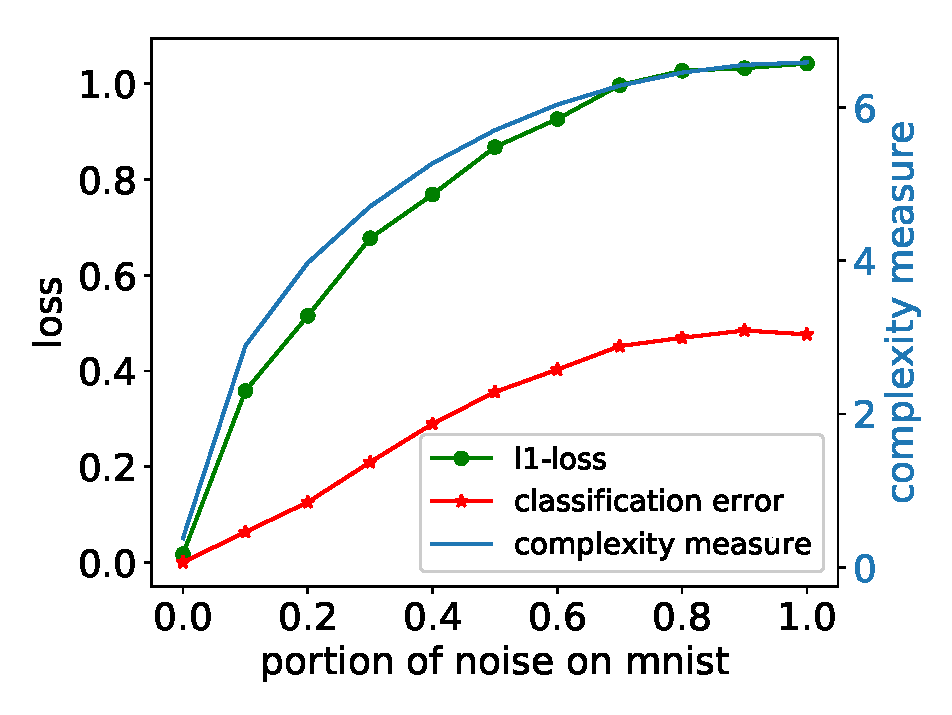
\includegraphics[width=0.4\textwidth]{figs/mnist_cm_noise.eps}}   
	\subfigure[CIFAR Data.]
	{
		\label{fig:generalization_cifar}
		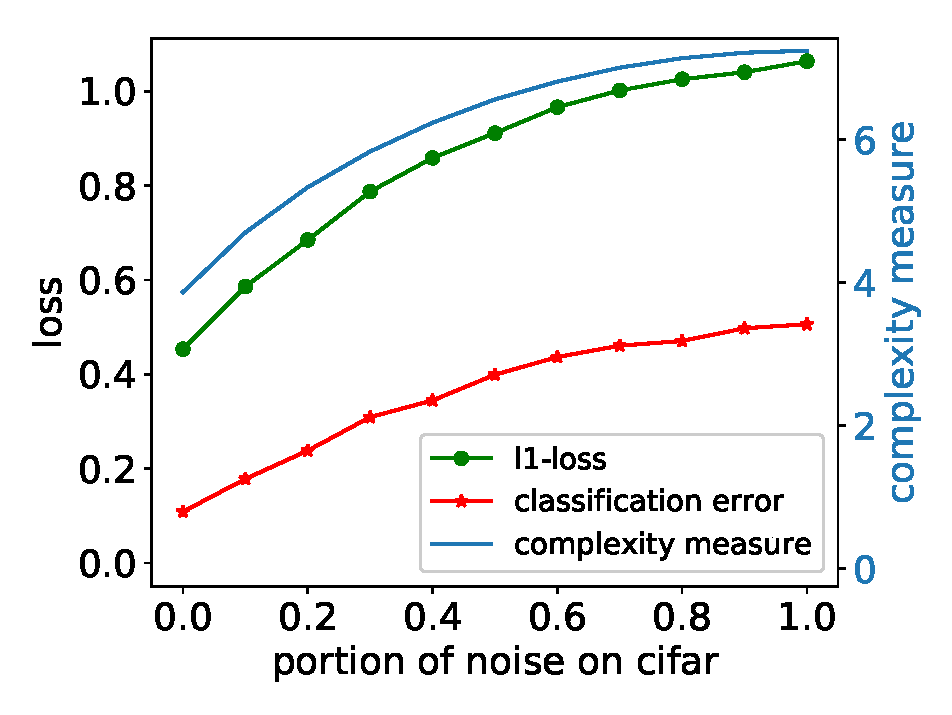
\includegraphics[width=0.4\textwidth]{figs/cifar_cm_noise.eps}}   
	\caption{Generalization error ($\ell_1$ loss and classification error) v.s. our complexity measure when different portions of random labels are used.
		%Comparison of generalization error using different portion of random labels. 
		We apply GD on data from two classes of MNIST or CIFAR until convergence.
			Our complexity measure almost matches the trend of generalization error as the portion of random labels increases.
			Note that $\ell_1$ loss is always an upper bound on the classification error.
		}
	\label{fig:generalization}
	\vspace{-0.5cm}
\end{figure}



\subsection{Proof Sketch of Theorem~\ref{thm:main_generalization}} \label{sec:proof_sketch_generalization}

The main ingredients in the proof of Theorem~\ref{thm:main_generalization} are Lemmas~\ref{lem:distance_bounds} and \ref{lem:rad_dist_func_class}. We defer the proofs of these lemmas as well as the full proof of Theorem~\ref{thm:main_generalization} to Appendix~\ref{app:proof_generalization}.

Our proof is based on a careful characterization of the trajectory of $\left\{\mat W(k) \right\}_{k=0}^\infty$ during GD.
In particular, we bound its \emph{distance to initialization} as follows:
\begin{lem}\label{lem:distance_bounds}
	Suppose $m \ge \kappa^{-2} \poly\left(n, \lambda_0^{-1}, \delta^{-1} \right)  $ and $\eta = O\left( \frac{\lambda_0}{n^2} \right)$.
	Then with probability at least $1-\delta$ over the random initialization, we have for all $k\ge0$:
	\begin{itemize}
		\item $\norm{\vect w_r(k) - \vect w_r(0)}_2 =O\left( \frac{ n }{\sqrt m \lambda_0\sqrt{\delta}} \right)$ $(\forall r\in[m])$, and
		%$\norm{\mat{W}(k) - \mat{W}(0)}_{2,\infty} \le \frac{\poly(n,1/\lambda_0)}{\sqrt{m}}$,
		\item $\norm{\mat{W}(k)-\mat{W}(0)}_{F} \le \sqrt{\vect{y}^\top \left(\mat{H}^{\infty}\right)^{-1}\vect{y}} + O\left( \frac{  n \kappa}{\lambda_0 \delta} \right) + \frac{\poly\left(n, \lambda_0^{-1}, \delta^{-1} \right)}{m^{1/4} \kappa^{1/2}} $.
		%\item $\norm{\mat{Z}(0)}_F \le \sqrt{\tr\left(\mat{H}^\infty\right)} + \frac{\poly(n,1/\lambda_0)}{\sqrt{m}}$.
	\end{itemize}
\end{lem}
The bound on the movement of each $\vect w_r$ was proved in \cite{du2018provably}. %and the bound on $\mat{Z}(0)$ is a simple application of Hoeffding inequality.
Our main contribution is the bound on $\norm{\mat{W}(k)-\mat{W}(0)}_F$ which corresponds to the \emph{total movement of all neurons}.
The main idea is to couple the trajectory of $\left\{\mat W(k) \right\}_{k=0}^\infty$ with another simpler trajectory $\left\{\widetilde{\mat{W}}(k)\right\}_{k=0}^\infty$ defined as:
%\begin{equation}
\begin{align}
\widetilde{\mat{W}}(0) =\,& \mat{0}, \nonumber\\
\vectorize{\widetilde{\mat{W}}(k+1)} =\,& \vectorize{\widetilde{\mat{W}}(k)} \label{eqn:W_tilde_traj} \\&- \eta\mat{Z}(0)\left( \mat{Z}(0)^\top \vectorize{\widetilde{\mat{W}}(k)}-\vect{y}\right). \nonumber
\end{align}
%\end{equation}
We prove $\norm{\widetilde{\mat W}(\infty) - \widetilde{\mat W}(0)}_F = \sqrt{\vect y^\top \mat H(0)^{-1} \vect y}$ in Section~\ref{sec:proof_sketch_distance}.\footnote{Note that we have $\mat H(0) \approx \mat H^\infty$ from standard concentration. See Lemma~\ref{lem:H(0)-H^inf}.}
The actually proof of Lemma~\ref{lem:distance_bounds} is essentially a perturbed version of this.


Lemma~\ref{lem:distance_bounds} implies that the learned function $f_{\mat W(k), \vect a}$ from GD is in a \emph{restricted} class of neural nets whose weights are close to initialization $\mat W(0)$.
The following lemma bounds the Rademacher complexity of this function class:
%We apply the generic Rademacher complexity method described in Section~\ref{sec:pre} to analyze the generalization ability.
%We consider the following function class.



%This functions in this class are two-layer neural networks with ReLU activation.
%The function class is defined a specific initialization $(\mat{W}(0), \vect{a})$ and two constants $R$ and $B$ that control the complexity of this function class.
%The only variable in this function class is the first layer weight matrix $\mat{W}$.
%Here $R$ controls its distance from $\mat{W}_0$ in $(2,\infty)$ norm and $B$ controls the distance in Frobenius norm.
%The next theorem bounds the Rademacher complexity of this function class.

\begin{lem}\label{lem:rad_dist_func_class}
%	For any fixed $\{\vx_i\}_{i=1}^n$ s.t. $\norm{\vx_i}\le 1$,$\forall i\in [n]$, suppose $\{\vw_r(0)\}_{r=1}^m$,$\{a_r\}_{r=1}^m$ are independently sampled from $N(\bm{0}, \initvar^2I_d)$, $\textrm{Unif}[-1,1]$ respectively. 
Given $R>0$,
with probability at least $1-\delta$ over the random initialization ($\mat W(0),\vect a)$, simultaneously for every $B>0$, the following function class
\begin{align*}
\cF^{\mat{W}(0),\va}_{R,B}  = \{ f_{\mat W, \vect a} : \norm{\vect w_r - \vect w_r(0)}_2 \le R \, (\forall r\in[m]), \\ \norm{\mat W - \mat W(0)}_F \le B \}
%&\cF^{\mat{W}(0),\va}_{R,B} = \{f:\reals^d \to \reals \mid f(\vx) = \sum_{r=1}^m\frac{ a_r}{\sqrt{m}} \relu{\vw_r^\top \vx}, \nonumber\\ &\quad \norm{\mat{W}(0)-\mat{W}}_{2,\infty}\le R,\norm{\vW(0)-\vW}_F\le B \}. \label{eqn:rad_func_class}
\end{align*}
has empirical Rademacher complexity bounded as:
%Then with high probability over the initialization the empirical Rademacher complexity has the following upper bound 
\begin{align*}
	&\calR_S\left( \cF^{\mat W(0),\va}_{R,B} \right)
   =  \frac{1}{n} \expect_{\bm \eps \in \{\pm1\}^n}\left[\sup_{f \in \cF^{\mat W(0),\va}_{R,B}}\sum_{i=1}^{n} \eps_i f(\vect{x}_i)\right]
	\\
	\le \,&	\frac{B}{\sqrt{2n}} \left(1+\left( \frac{2\log \frac2\delta}{m} \right)^{1/4} \right) + \frac{2 R^2 \sqrt m}{ \kappa} + R \sqrt{2\log \frac2\delta} .
\end{align*}
\end{lem}

Finally, combining Lemmas~\ref{lem:distance_bounds} and \ref{lem:rad_dist_func_class}, we are able to conclude that the neural network found by GD belongs to a function class with Rademacher complexity at most $\sqrt{\vect y^\top (\mat H^\infty)^{-1} \vect y /(2n)}$ (plus negligible errors).
This gives us the generalization bound in Theorem~\ref{thm:main_generalization} using the theory of Rademacher complexity (Appendix~\ref{app:rademacher}).

%Lemma~\ref{lem:rad_dist_func_class} is related to 
%inspired by recent works by~\citep{behnam,vashnav} who also used the distance from initialization to characterize the complexity of the function class.
%The key difference here is that we use both $(2,\infty)$ norm and Frobenius norm to control the complexity.
%The proof is thus more involved than previous papers and we refer readers to appendix for the whole proof.


%While Theorem~\ref{thm:rad_dist_func_class} and Rademacher complexity bounds in ~\citep{behnam,vashnav} induce new generalization bounds that depend on the distance from the initialization, these only account for half of the generalization story, i.e., we do not know when the distance is large and when the distance is small.
%Using the idea developed in this paper, by analyzing the trajectory of $\mat{W}(k)$, we are able to complete the story.
%The following theorem gives bounds on $B$, $R$ and $\norm{\vZ(0)}_F$.




%Now combining Theorem~\ref{thm:rad_generalization},~\ref{thm:rad_dist_func_class} and~\ref{thm:distance_bounds}, we obtain our final generalization result in this paper.






\subsection{Analysis of the Auxiliary Sequence $\left\{\widetilde{\mat{W}}(k)\right\}_{k=0}^\infty$}
\label{sec:proof_sketch_distance}
Now we give a proof of  $\norm{\widetilde{\mat W}(\infty) - \widetilde{\mat W}(0)}_F = \sqrt{\vect y^\top \mat H(0)^{-1} \vect y}$ as an illustration for the proof of Lemma~\ref{lem:distance_bounds}.
Define $\vect v(k) = \mat Z(0)^\top \vectorize{\widetilde{\mat W}(k)} \in \R^n$.
Then from~\eqref{eqn:W_tilde_traj} we have $\vect v(0)=\vect0$ and $\vect v(k+1) = \vect v(k) - \eta \mat H(0) (\vect v(k) - \vect y)$, yielding
$\vect v(k) - \vect y = - (\mat I - \eta \mat H(0))^k \vect y$.
Plugging this back to~\eqref{eqn:W_tilde_traj} we get
$\vectorize{\widetilde{\mat{W}}(k+1)} - \vectorize{\widetilde{\mat{W}}(k)} = \eta \mat Z(0) (\mat I - \eta \mat H(0))^k \vect y$.
Then taking a sum over $k=0, 1, \ldots$ we have
\vspace{-0.2cm}
\begin{align*}
\vectorize{\widetilde{\mat{W}}(\infty)} - \vectorize{\widetilde{\mat{W}}(0)} &= \sum_{k=0}^\infty \eta \mat Z(0) (\mat I - \eta \mat H(0))^k \vect y \\
&= \mat Z(0) \mat H(0)^{-1} \vect y.
\end{align*}
\vspace{-0.2cm}
The desired result thus follows:
\begin{align*}
\norm{\widetilde{\mat W}(\infty) - \widetilde{\mat W}(0)}_F^2
&= \vect y^\top \mat H(0)^{-1} \mat Z(0)^\top \mat Z(0) \mat H(0)^{-1} \vect y \\
&= \vect y^\top \mat H(0)^{-1} \vect y.
\end{align*}



%Again note $\left\{\mat{W}(k)\right\}_{k=0}^\infty$ and $\left\{\widetilde{\mat{W}}(k)\right\}_{k=0}^\infty$ have the same initialization but $\left\{\widetilde{\mat{W}}(k)\right\}_{k=0}^\infty$ only uses a fixed initial extended feature matrix $\mat{Z}(0)$ to do the update whereas $\left\{\widetilde{\mat{W}}(k)\right\}_{k=0}^\infty$ depends on $\mat{Z}(0)$ which varies at each iteration.
%Equivalently, one can view $\left\{\widetilde{\mat{W}}(k)\right\}_{k=0}^\infty$ is generated according to applying gradient descent on the loss $\frac{1}{2}\norm{\mat{Z}(0)^\top \vectorize{\widetilde{\mat{W}}(k)}-\vect{y}}_2^2$.

%
%
%We have the following results.
%\begin{thm}\label{thm:W_distance}
%\begin{align*}
%\norm{\mat{W}(k)-\mat{W}(0)}_F^2 \le \vect{y}^\top \mat{H}^\infty \vect{y} + \frac{\poly(n,1/\lambda_0)}{\sqrt{m}}
%\end{align*}
%\end{thm}
%\begin{proof}[Proof of Theorem~\ref{thm:W_distance}]
%We consider gradient flow:
%\begin{align*}
%\frac{d \mat W(t)}{dt} = - \nabla L(\mat W(t)).
%\end{align*}
%
%We have
%\begin{equation*}
%\frac{d \vect u(t)}{dt} = - \mat H(t) \cdot \left( \vect u(t) - \vect y \right).
%\end{equation*}
%
%
%
%
%
%When $m$ is sufficiently large, we know $\mat H(t) \approx \mat H(0) \approx \mat H^\infty$ and $\mat Z(t) \approx \mat Z(0)$.
%
%Take SVD: $$\mat Z(0) = \sum_{i=1}^{n} \sigma_i \vect u_i \vect v_i^\top$$ and EGD: $$\mat H(0) = \sum_{i=1}^{n} \lambda_i \vect v_i \vect v_i^\top.$$ Here $\lambda_i = \sigma_i^2$.
%
%
%Write 
%\begin{align*}
%\vect u(0) - \vect y = \sum_{i=1}^{n} c_i \vect v_i.
%\end{align*}
%From $\frac{d \vect u(t)}{dt} \approx - \mat H(0) \cdot \left( \vect u(t) - \vect y \right)$ we get
%\begin{align*}
%\vect u(t) - \vect y \approx \sum_{i=1}^{n} e^{-\lambda_i t} c_i \vect v_i.
%\end{align*}
%Then
%\begin{equation*}
%\begin{aligned}
%vec\left( \frac{d \mat W(t)}{dt} \right) &= -vec\left( \nabla L(\mat W(t)) \right) =  -\mat Z(t)\cdot (\vect u(t) - \vect y) \\
%& \approx -\mat Z(0) \cdot \sum_{i=1}^{n} e^{-\lambda_i t} c_i \vect v_i \\
%&= - \sum_{i=1}^{n} \sigma_i \vect u_i \vect v_i^\top \cdot \sum_{i=1}^{n} e^{-\lambda_i t} c_i \vect v_i \\
%&=  - \sum_{i=1}^{n} e^{-\lambda_i t} c_i \sigma_i \vect u_i .
%\end{aligned}
%\end{equation*}
%Therefore
%\begin{equation*}
%\begin{aligned}
%&\norm{\mat W(\infty) - \mat W(0)}_F\\
%&= \norm{\int_{0}^{\infty} \frac{d \mat W(t)}{dt} dt}_F
%= \norm{\int_{0}^{\infty} vec\left( \frac{d \mat W(t)}{dt} \right) dt}\\
%&\approx \norm{\int_{0}^{\infty} \left( \sum_{i=1}^{n} e^{-\lambda_i t} c_i \sigma_i \vect u_i \right)  dt}\\
%&= \norm{\sum_{i=1}^{n} \frac{1}{\lambda_i} c_i \sigma_i \vect u_i } 
%= \sqrt{\sum_{i=1}^n \left( c_i \sigma_i / \lambda_i \right)^2} 
%= \sqrt{\sum_{i=1}^n  \frac{c_i^2}{\lambda_i}} \\
%&= \sqrt{ \left( \vect u(0) - \vect y \right)^\top \left(\mat H(0)\right)^{-1} \left( \vect u(0) - \vect y \right) }.
%\end{aligned}
%\end{equation*}
%\end{proof}


%\begin{proof}[Proof of Theorem~\ref{thm:generalization}]
%First we consider the function class \[\cF_M = \left\{f(\mat{W},\vect{a},\vect{x}) = \frac{1}{\sqrt{m}}\sum_{r=1}^{m}a_r\relu{\vect{w}_r^\top \vect{x}}, \norm{\mat{W}-\mat{W}_0}_F \le M \right\}.\]
%Its empirical Rademacher complexity is defined as \begin{align*}
%	\bar{\mathcal{R}}_n(\cF_M) = \expect_{\epsilon_i \sim \unif\left[\left\{-1,1\right\}\right]}\sup_{g \in  \cF_M}\sum_{i=1}^{n}\epsilon_ig(\vect{x}_i).
%\end{align*}
%We can bound it by \begin{align*}
%	&\bar{\mathcal{R}}_n(\cF_M)  \\
%	=&\expect_{\epsilon_i \sim \unif\left[\left\{-1,1\right\}\right]}\sup_{\norm{\mat{W}-\mat{W}_0}_F \le M}\sum_{i=1}^{n}\epsilon_i f(\mat{W},\vect{a},\vect{x}_i)\\
%	=&\expect_{\epsilon_i \sim \unif\left[\left\{-1,1\right\}\right]}\sup_{\norm{\mat{W}-\mat{W}_0}_F \le M}\sum_{i=1}^{n}\epsilon_i f(\mat{W}_0,\vect{a},\vect{x}_i)\\
%	& + \expect_{\epsilon_i \sim \unif\left[\left\{-1,1\right\}\right]}\sup_{\norm{\mat{W}-\mat{W}_0}_F \le M}\sum_{i=1}^{n}\epsilon_i \left(f(\mat{W}_0,\vect{a},\vect{x}_i)-f(\mat{W}_0,\vect{a},\vect{x}_i)\right) \\
%	= & \expect_{\epsilon_i \sim \unif\left[\left\{-1,1\right\}\right]}\sup_{\norm{\mat{W}-\mat{W}_0}_F \le M}\sum_{i=1}^{n}\epsilon_i \left(f(\mat{W}_0,\vect{a},\vect{x}_i)-f(\mat{W}_0,\vect{a},\vect{x}_i)\right) \\
%	= & \expect_{\epsilon_i \sim \unif\left[\left\{-1,1\right\}\right]}\sup_{\norm{\mat{W}-\mat{W}_0}_F \le M}\sum_{i=1}^{n}\epsilon_i \frac{1}{\sqrt{m}}\sum_{r=1}^{m}a_r \left(\relu{\vect{w}_r^\top\vect{x}_i} - \relu{\vect{w}_{0,r}^\top \vect{x}_i}\right)
%	\end{align*}
%\end{proof}


%Let 
%\begin{itemize}
%\item $\mu$ be the standard Gaussian measure in $\reals^d$;
%\item $f: \reals^d \times \reals^+ \to \reals^d$ be the parameters of the network;
%\item $X\in \reals^{d\times n}$ be the data matrix where the the $i$th column $\bx_i$ is the $i$th feature;
%\item the feature map $X(\bw)$ is defined as  $\left[\bx_1\bone[\bx_1^T\bw\geq 0],\bx_2\bone[\bx_2^T \bw\geq 0], \ldots, \bx_n\bone[\bx_n^T \bw\geq 0]\right]$;
%\item the vector $\by\in\reals^d$ be the true labels;
%\item the prediction $\bu(t)=\E_{\bw\sim \mu}X^\top(\bw)f(\bw,t)$ and the difference $\bz(t) = \by-\bu(t)$.
%\item the kernel $H_n = \E_{\bw\sim \mu} X^\top(\bw)X(\bw)$.
%\end{itemize}
%
%Suppose $f$ satisfies the following euqaiton:
%\begin{align} 
%\frac{\partial f(\bw,t)}{\partial t} =& X(\bw)(\by-\bu(t))\label{eq:dynamic_w}\\
% \qquad  f(\bw,0)=&\mathbf{0}, \forall \bw \in \reals^d,
% \end{align}
%
%then we have 
%
%\[ \| f(w,\infty)\|^2_{L_2(\mu)} = \E_{\bw\sim \mu} \|f(w,\infty)\|_2^2  = \by^\top H_n^{-1}\by.\]
%
%
%\begin{proof}
%By definition of $\bz(t), \bu(t)$ and \eqref{eq:dynamic_w}, we have 
%
%\[\frac{d\bz(t)}{dt}  = -\frac{d\bu(t)}{dt} = -\E_{\bw\sim \mu}X^\top(\bw)\frac{\partial f(\bw,t)}{\partial t}= -\E_{\bw\sim \mu}X^\top(\bw)X(\bw)(\by-\bu(t))=-H_n\bz(t).\]
%
%Integrate both sides and note that $\bz(\infty) = 0$, we have 
%\[\int_{t=0}^\infty \bz(t) = -H_n^{-1} \int_{t=0}^\infty \frac{d\bz(t)}{dt} = H_n^{-1} (\bz(0)-\bz(\infty))= H_n^{-1}\bz(0).\]
%
%Thus,  
%\[f(\bw,\infty) = \int_{t=0}^\infty \frac{\partial f(\bw,t)}{\partial t}dt =  - \int_{t=0}^\infty X(\bw)\bz(t) dt = -X(\bw)H_n^{-1}\bz(0),\]
%
%which implies
%
%\[\E\limits_{\bw\sim \mu} \|f(w,\infty)\|_2^2 = E_{\bw\sim \mu} \bz(0) H_n^{-1} X^\top(\bw)X(\bw)H_n^{-1}\bz(0) = \bz(0)H_n^{-1}\bz(0) = \by^\top  H_n^{-1}\by\]
%
%\end{proof}
%
%For  function class $\mathcal{G}:= \{g(\bx)| g(\bx) = \E_{w\sim \mu} f(\bw)^\top x\ \bone[\bw^\top \bx\ge 0], \E_{\bw\sim \mu}\|f(\bw)\|_2^2\le C^2)\} $, its empirical rademacher complexity is defined as 
%\[\rc{\mathcal{G}} = \E_{\beps\sim \{\pm 1\}^n}\sup_{g\in \mathcal{G}} \sum_{i=1}^n \eps_i g(\bx_i).\]
%
%\begin{theorem}
%\[\rc{\calG} \leq C \|X\|_F.\]
%\end{theorem}
%
%\begin{proof}
%\begin{equation}
%\begin{split}
%\rc{\mathcal{G}} 
%=& \E_{\beps\sim \{\pm 1\}^n}\sup_{g\in \mathcal{G}} \sum_{i=1}^n \eps_i g(\bx_i)\\
%=& \E_{\beps\sim \{\pm 1\}^n}\sup_{\|f\|_{L_2(\mu)\le C}} \E_{\bw\sim \mu} \beps^\top X(\bw)f(\bw)\\
%= &\E_{\beps\sim \{\pm 1\}^n}C\sqrt{ \E_{\bw\sim \mu} \|\beps^\top X(\bw)\|_2^2}\\
%\leq & C \sqrt{\E_{\beps\sim \{\pm 1\}^n} \E_{\bw\sim \mu} \|\beps^\top X(\bw)\|_2^2}\\
%= & C \sqrt{\E_{\beps\sim \{\pm 1\}^n} \beps^\top H_n \beps}\\
%= &C \sqrt{\trace(H_n)}\\
%= & \frac{C}{2} \|X\|_F
%\end{split}
%\end{equation}
%
%\end{proof}
%
%\begin{lem}\label{lem:inv_psd}
%For any $A,B\in \reals^{n\times n}$, $B\succeq A\succeq 0$, we have $A^\dag\succeq P_A B^\dag P_A$, where $P_A = A^{1/2}A^\dag A^{1/2}$ is the projection matrix for the subspace spanned by $A$ .\footnote{$A^\dag$ is the pseudo inverse of $A$.}
%
%Note that when $A$,$B$ are all inversible,  the result is just $A^{-1}\succeq B^{-1}$.
%\end{lem}
%
%\begin{proof}
%W.l.o.g, we can assume $B$ is inversible, namely $B^{-1}=B^{\dag}$. Additionally, we can assume $A$ is diagonal and $A= \begin{pmatrix}\Sigma &0 \\0& 0\end{pmatrix} $. Thus $P_
%A =  \begin{pmatrix}I_A &0 \\0& 0\end{pmatrix}$ and $P_A^\perp = I-P_A =\begin{pmatrix}0 &0 \\0& I\end{pmatrix}$. 
%
%Now we will show that all roots of equation $\det(P_AB^{-1}P_A-\lambda (A^\dag + P_A^\perp))=0$ are between $0$ and $1$, which would imply $A^\dag \succeq P_AB^{-1}P_A$.
%
%Note that 
%\begin{equation}
%\begin{split}
%&\det(P_AB^{-1}P_A-\lambda (A^\dag + P_A^\perp)) \\
%=& \det(B^{-1}P_A-\lambda (A^\dag + P_A^\perp)) \\
%=& \det(B^{-1})\det(P_A-\lambda B(A^\dag + P_A^\perp))\\
%= &\det(B^{-1})\det((A-\lambda B)(A^\dag + P_A^\perp))\\ 
%= &\det(B^{-1})\det(A^\dag + P_A^\perp)\det(A-\lambda B),\\
%\end{split}
%\end{equation}
%
%and $\det(B^{-1})>0, \det(A^\dag + P_A^\perp)>0$,  the roots of equation $\det(P_AB^{-1}P_A-\lambda (A^\dag + P_A^\perp))=0$ are exactly the roots of $\det(A-\lambda B)=0$. Since $B\succeq A\succeq 0$, $\det(A-\lambda B)\neq 0 $ when $\lambda<0$ or $\lambda >1$.
%\end{proof}
%\begin{theorem}
%If $y_i=\balpha^\top \bx_i,\ \forall 1\in[n]$, then $\E_{\bw\sim \mu} \|f(w,\infty)\|_2^2 \leq \frac{\|\balpha\|_2^2}{4}$.
%\end{theorem}
%
%
%
%
%\begin{proof}
%
%Define $k(\bx,\bx') = \frac{\bx^\top \bx'}{\|\bx\|_2\|\bx'\|_2}$, $H(\bx,\bx') = \bx^\top \bx'\left(\frac{\arcsin\frac{\bx^\top \bx'}{ \|\bx\|_2\|\bx'\|_2}}{2\pi}+\frac{1}{4}\right) = \|\bx\|_2\|\bx'\|_2 k(\bx,\bx')\left(\frac{\arcsin k(\bx,\bx')}{2\pi}+\frac{1}{4}\right)$.
%
%By cite[kernel methods in deep learning], we have $H_n^{ij} = H(\bx_i,\bx_j)$. Taking Taylor expansion of $\arcsin$, we know $H_n \succeq \frac{X^\top X}{4}$. Additionally,  $P_X = X^\top (XX^\top)^\dag X$ is a  projection matrix, because $P_X^2  = X^\top (XX^\top)^\dag (XX^\top)(XX^\top)^\dag X = X^\top (XX^\top)^\dag X = P_X$.  Moreover, $P_X =  \sqrt{X^\top X} (X^\top X)^\dag \sqrt{X^\top X}$, thus we can apply Lemma~\ref{lem:inv_psd}.
%
%\[ \E_{\bw\sim \mu} \|f(w,\infty)\|_2^2 = \by^\top H_n^{-1} \by =\balpha^\top X H_n^{-1} X^\top \balpha = \balpha^\top X P_XH_n^{-1}P_X X^\top \balpha \le \balpha^\top X (X^\top X)^\dag X^\top \balpha /4.\]
%
%By the same argument, we can show $X (X^\top X)^\dag X^\top$ is a projection matrix, thus 
%
%\[\E_{\bw\sim \mu} \|f(w,\infty)\|_2^2 = \balpha^\top X (X^\top X)^\dag X^\top \balpha /4 \le \frac{\|\balpha\|_2^2}{4}.\]
%
%
%\end{proof}
%
%\begin{thm}
%Fix distribution D on domain $\reals^d$, $\balpha \in \reals^d$ and parameter $\delta\in [0,1]$, if $S = \{\bx_1,\bx_2,\ldots,\bx_n\}$ are sampled i.i.d. from $D$,  and $y_i=\balpha^\top \bx_i,\ \forall i\in [n]$, then for any  loss function $l(\cdot,\cdot): \reals\times\reals \to \reals$ which is $L$- lipschitz in the first parameter, the output function of the kernel at $t=\infty$, i.e., $g(\bx) = \E_{\bw\sim \mu}f(\bw,\infty)^\top \bx \bone[\bx^\top \bx\ge 0]$, satisfies the following property: 
%
%W.p. $1-\delta$, 
%
%\[\E_D \left[l(g(\bx),\balpha^\top \bx)\right] \leq \E_S \left[l(g(\bx),\balpha^\top \bx)\right] + \frac{L\|\balpha\|_2\|X\|_F}{2n} + \sqrt{\frac{\ln\frac{1}{\delta}}{n}}.\]
%\end{thm}